
\subsection{Functional requirements}
We assume that all domain properties stipulated in paragraph 1.6 hold. We decided to use a \textit{goal-driven} method to structure our requirements, meaning that we decomposed the high-level goals of paragraph 1.5 into low-level requirements.
Some of these requirements stem directly from the requests of our clients, while others are born from the necessity to have a sound system.

For each goal, we derive the following requirements:


%MEDIUM LEVEL
\begin{itemize}


				\item [G1] Registration procedure %The system allows guests to register; to complete the registration procedure the system sends a password to the guest as an access key.
					\begin{itemize}
						\item The system has to allow any person to sign up.
						\item The system has to send a newly generated password to the user via email when prompted by the admin.
						\item The system must be able to check whether a password is correct or not.
						\item The system must let the user log in only if the password is correct. 
					\end{itemize}
				\item [G2] Localization %The system should be able to locate the users once they have given their permission.
					\begin{itemize}
						\item The system must be able to locate the user through their smartphone's GPS with sufficient precision.
						\item The system must locate the user if and only if they have given their permission. 
					\end{itemize}
				\item [G3] Finding cars %The system should enable a registered user to find the location of an available car within a certain distance from the user's location or from a specified address.
					\begin{itemize}
						\item The system must be able to find any specific address on the city map. %FIXME horridly put.
						\item The system must be able to find parking areas in a given area of the map. 
						\item The system must be able to identify available cars inside parking areas.
						\item The system must let users see whether there are available cars in a specified radius. 
					\end{itemize}
				\item [G4] Services provided %The system enables user to reserve a single available car in a certain geographical region for one hour before the user picks it up. If the car is not picked up by that time, the reservation expires, the system tags this car as available again and it charges the user a fine of 1 EUR.
					\begin{itemize}
						\item The system must allow users to reserve an available car.
						\item The cars cannot be reserved by more than one user at any given time.
						\item The system must keep the current reservation standing until the user has opened the car or an hour has passed.
						\item The system must be able to autonomously cancel reservations.
						%TODO others?
					\end{itemize}
				\item [G5] Knowledge of the cars %The system should keep track of every activity within the cars of PowerEnJoy, by means of sensors and tracking devices, i.e. location, battery charge, health status, number of passengers. 
					\begin{itemize}
						\item The system must be able to locate any car at any given time with sufficient precision.
						\item The system must be able to detect whether there are passengers inside a car, and how many.
						\item The system must be able to collect data about the power charge of any of its cars.
						\item The system must be able to detect when a severe accident has occurred to a car. %too much?
						\item The system must be able to detect when a user is near a car through the car's (and the user's mobile phone's) bluetooth system.
						\item The system must be able to tell when a car is parked in a safe area.
						\item The system must be able to detect when a car is plugged to the power grid.
						\item The system must be able to detect whether the driver is still in the car.
					\end{itemize}
				\item [G6] Control of the cars %The system should be able to command remotely and automatically some of the features of the cars, for example locking and unlocking the doors. 
					\begin{itemize}
						\item The system must be able to automatically unlock a car when the user that has reserved it is nearby.
						\item The system must be able to automatically lock a car when the user has exited it inside a safe area. 
					\end{itemize}
				\item [G7] Charges %The system charges the user for a predefined amount of money per minute. A screen on the car notifies the user of the current charges.
					\begin{itemize}
						\item The system must be able to calculate the fee to charge the user.
						\item The system should notify the user of the fee per minute he's being charged through a screen inside the car.
					\end{itemize}
				\item [G8] Boundaries of charges %The system starts charging the user as soon as the car ignites. It stops charging them when the car is parked in a safe area and the user exits the car. The user must confirm the operation, otherwise the system keeps charging them. 
					\begin{itemize}
						\item The system must be able to tell when the car has ignited. 
						\item The system should start counting the charges from the ignition onward. %FIXME horridly put and don't know if a requirement.
						\item The system must ask the user whether they wish to end the ride or not as soon as they are parked in a safe area and have exited the car; if they decide so, the system should stop charging them, otherwise it should keep doing so. 
					\end{itemize}
				\item [G9] Discounts and sanctions %The system should encourage good user behaviour and discourage bad behaviour through the application of discounts and sanctions to the fee per minute. 
					\begin{itemize}
						\item The system must apply a discount every time a user brings two or more passengers in the car with them.
						\item The system must apply a discount every time the car has more than 50\% of power charge by the end of the ride. %FIXME horridly put
						\item The system must be able to apply a discount every time the user plugs the car in the power grid as soon as they're finished using the car. %FIXME: 10 minutes window here?
						\item The system must apply a sanction every time a car is returned in a safe area at more than 3 km from the nearest recharging safe area.
						\item The system must apply a sanction every time a car is returned with less than 20\% of power charge.
						\item The system must provide an option (\textit{money saving}) to get information about the best safe area where the user can leave the car so that an uniform distribution of cars among the city is distributed. 
						\item The system	 must be able to compute which is the best safe area for a user with \textit{money saving} activated according to their destination and the nature of the safe areas (recharging or not).	 %are the last two clear???			
						\item The system must apply a discount every time the car is returned in the suggested safe area with the \textit{money saving} option.
					\end{itemize}
				\item [G10] Emergency management %The system keeps a channel of communication open between the users and the administrators of the system in case of emergencies. 
					\begin{itemize}
						\item The system must always allow a user to notify the back-end administrators if they have a problem with the car.
						\item The system must be able to locate \textit{PowerEnJoy} operators in order to facilitate their quick dispatch.
					\end{itemize}

\end{itemize}












%VERY LOW LEVEL
%not finished

\begin{itemize}

	%Pat's goals
	
	\item [G1] Registration of a guest to the system.%\textbf{G1} Guest are able to register to the System. Each guest must fill a profile to become a user.
		\begin{itemize}
			\item The system has to allow any person to sign up. 
		\end{itemize}
	\item [G2] Access to the system %\textbf{G2} To complete the procedure of registration the system sends a password to the guest as an access key.
		\begin{itemize}
			\item The system has to send a newly generated password to the user via email when prompted by the admin.
			\item The system must be able to check whether a password is correct or not.
			\item The system must let the user log in only if the password is correct. 
		\end{itemize}
	\item [G3] Finding cars % \item \textbf{G3} The system enables the registered user to find the locations of an available car within a certain distance from the user's location or from a specified address.
		\begin{itemize}
			\item The system must be able to locate the user through their smartphone's GPS.
			\item The system must be able to find a specific address in its map. %FIXME horridly put.
			\item The system must be able to find parking areas in a given area of the map. 
			\item The system must be able to identify available cars inside parking areas.
			\item The system must let users see whether there are available cars in a specified radius. 
		\end{itemize}
	\item [G4] Reservation of a car %The system enables user to reserve a single available car in a certain geographical region for one hour before the user picks it up.
		\begin{itemize}
			\item The system must allow users to reserve an available car.
			\item The cars cannot be reserved by more than one user at any given time.
			\item The system must keep the current reservation standing until the user has opened the car or an hour has passed.
		\end{itemize}
	\item [G5] Fine for not picking up a reserved car. % If the reserved car is not picked up within one hour from the reservation time, the reservation expires and the system tag this car as available. The system charges user a fee of 1 EUR. 
		\begin{itemize}
			\item The system must be able to cancel reservations.
			%TODO others?????
		\end{itemize}
	\item [G6] Opening a car %When the user tells the system that he's near the reserved car, the system unlocks the car to let the user enter.  
		\begin{itemize}
			\item The system should be able to detect when a user is near a reserved car throught the car's Bluetooth system.
			\item The system should be able to unlock a specific car.
		\end{itemize}
	
	
	%Mad's goals	
	
	\item [G7] Charging fees to the user %The system charges the user for a predefined amount of money per minute.
		\begin{itemize}
			\item The system must be able to calculate the fee to charge the user.
			\item The system should notify the user of the fee per minute he's being charged.
		\end{itemize}
	\item [G8] Starting charging %The system starts charging the user as soon as the car ignites.
		\begin{itemize}
			\item The system must be able to tell when the car has ignited. 
			\item The system should start counting the charges from the ignition onward. %FIXME horridly put and don't know if a requirement.
		\end{itemize}
	\item [G9] Ending charging %The system stops charging the user when the car is parked in a safe area and the user exits the car. The user must confirm the operation, otherwise the system keeps charging them. 
		\begin{itemize}
			\item The system must be able to tell when the car is parked in a safe area.
			\item The system must be able to detect whether the driver is still in the car.
			\item The system must ask the user whether they wish to end the ride or not as soon as they are parked in a safe area and have exited the car; if they decide so, the system should stop charging them, otherwise it should keep doing so. 
		\end{itemize}
	\item [G10] Notification of the current charges %A screen on the car notifies the user of the current charges.
		\begin{itemize}
			\item The system must calculate the charges in real time. %DAMMIT this is heinous. 
			\item The system should show the current charges onscreen. 
		\end{itemize}
	\item [G11] Locking a car %The system locks the car automatically when the user exits the car inside a safe area.
		\begin{itemize}
			\item The system should be able to lock a specific car without user input. %FIXME is "without user input" correct?
			%all other points (inside safe area and user still inside) already written in [G9]
		\end{itemize}
	\item [G12] %not sure if a goal after all
	\item [G13] Time window %If the user has chosen to stop being charged, the system keeps a 10–minutes window of time when they are allowed to re-open the car if it has not already been reserved by someone else.
		\begin{itemize}
			\item The system must allow the last user who has driven a car to unlock and open it within a 10-minutes window and if and only if the car has not already been reserved by someone else.
			\item The system must not allow more than one user at a time to open a car.
		\end{itemize}
	\item [G14] Parking areas %The set of safe parking areas is pre–defined by the management system.
		\begin{itemize}
			\item The system must know the location of all parking areas at any given time. 
		\end{itemize}
	\item [G15] Passenger's discount %The system allows the user to earn a 10\% discount for the current ride if there are at least two other passengers in the car.
		\begin{itemize}
			\item The system must be able to detect how many passengers are in the car through specific sensors.
			\item The system must be able to apply a discount to every ride where there are two or more passengers in the car.
		\end{itemize}
	
	
	%Poe's goals
	
	\item [G16] Discount for power charge %The system applies a 20\% discount on the current ride if the car is returned by the user with more than 50\% of power charge.
		\begin{itemize}
			\item The system must be able to apply a discount on every ride when the car has more than 50\% of power charge by the end of the ride. %FIXME horridly put
			\item The system must be able to collect data about the power charge of any car.
		\end{itemize}
	\item [G17] Discount for plugging the car to the power grid %If a user returns a car to a recharging safe area and plugs it into the power grid, the system applies a 30\% discount on his current ride.
		\begin{itemize}
			\item The system must be able to discern whether a car is currently plugged in to the power grid and is being recharged.
			\item The system must be able to apply a discount on every ride if the user plugs the car in the power grid as soon as they're finished. %FIXME: 10 minutes window? Change the goal? 
		\end{itemize}
	\item [G18] Sanction for distance %The system applies a 30\% sanction on the current ride if the car is returned in a safe area at more than 3 km from the nearest recharging safe area.
\end{itemize}



\subsection{Non-functional requirements}
	\subsubsection{User interface}
	\paragraph{}The interface of our application is thought to be used mainly via mobile app, with some content also displayed in a web page. The team reasoned that the main functionalities of the system (such as reserving and managing a car) make sense only in a \textit{movable} context (meaning, such that the user can do them anywhere they have an internet connection). Those functionalities are available on the mobile app. On the other hand, operations such as signing up are more easily managed in front of a computer, so the web page allows users to register, login and manage their profiles (which they can do also via mobile app anyway).
	\paragraph{}We pondered on the possibility of adding the possibility of reserving a car via web browser. However, upon consideration, we decided it is not a good mechanism: with that functionality, a user could very well be registered without having downloaded the app and reserving a car without being able to access it in any way. Hence, the reservation of \textit{PowerEnJoy} cars can be made only via mobile app. 
	
	\paragraph{Mobile app}\mbox{}\\
	
	\begin{figure}[h]
 
		\begin{subfigure}{0.5\textwidth}
			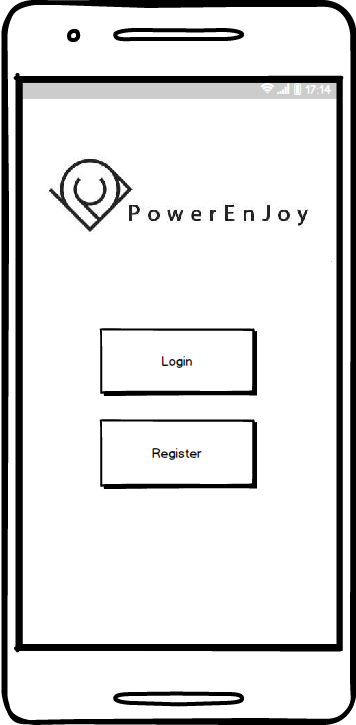
\includegraphics[scale=0.35]{img/mockups/App_guest.png}
			\caption{Guest view}
			\label{fig:subim1}
		\end{subfigure}
		\begin{subfigure}{0.5\textwidth}
			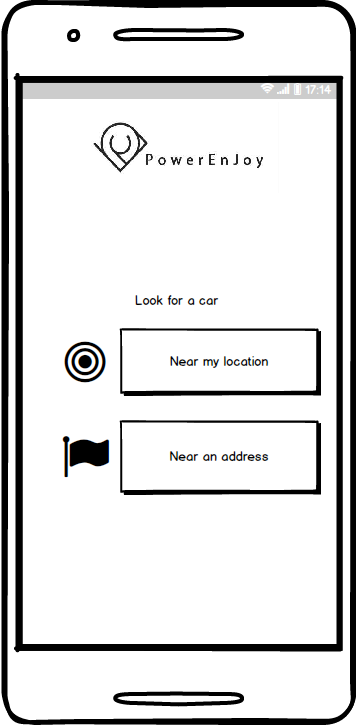
\includegraphics[scale=0.35]{img/mockups/App_user.png}
			\caption{User view}
			\label{fig:subim2}
		\end{subfigure}
 
		\caption{Mobile app: home page view}
		\label{fig:image1}
	\end{figure}
	
	\paragraph{} Figure 1 shows the first page that is shown when entering the app. Picture 1.a is the guest view, who has only the possibility of either logging in or registering in the system. Picture 1.b shows the user view. The user has more functionalities: they can look for cars in their vicinity or near an address, see and edit their profile, and changing settings (notification and sound settings). 
	
	\begin{figure}[h]
 
		\begin{subfigure}{0.3\paperwidth}
			\centering
			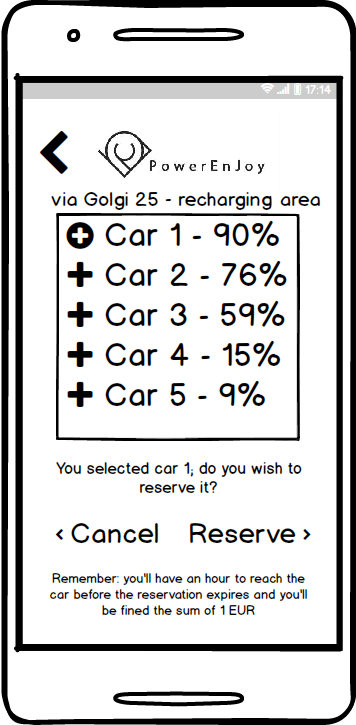
\includegraphics[scale=0.35]{img/mockups/User_reservation.png}
			\caption{View for the reservation}
			\label{fig:subim1}
		\end{subfigure}
		\begin{subfigure}{0.3\paperwidth}
			\centering
			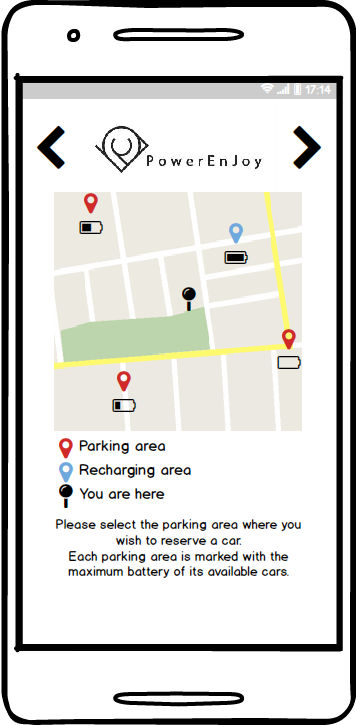
\includegraphics[scale=0.35]{img/mockups/User_parking_areas.png}
			\caption{View after having selected a parking area}
			\label{fig:subim2}
		\end{subfigure}
		\begin{subfigure}{0.3\paperwidth}
			\centering
			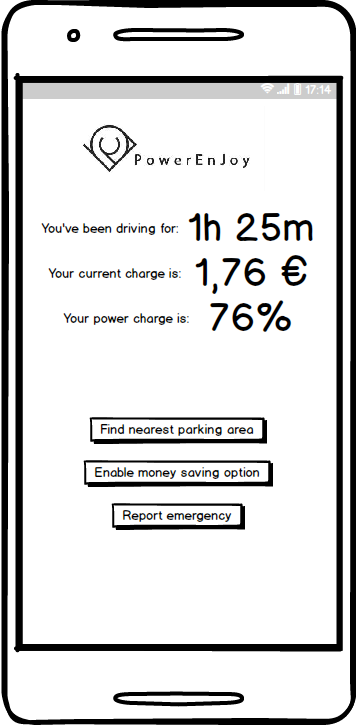
\includegraphics[scale=0.35]{img/mockups/User_driving.png}
			\caption{Display of the app while using a car}
			\label{fig:subim3}
		\end{subfigure}
 		
		
		\caption{Mobile app: main functionalities}
		\label{fig:image2}
	\end{figure}
	
	\paragraph{} Figure 2 shows the main functionalities of the \textit{PowerEnJoy}'s app: reserving a car (2.a and 2.b) and what you can do while using a car (2.c). 
	
	\begin{figure}
		\begin{subfigure}{1\textwidth}
			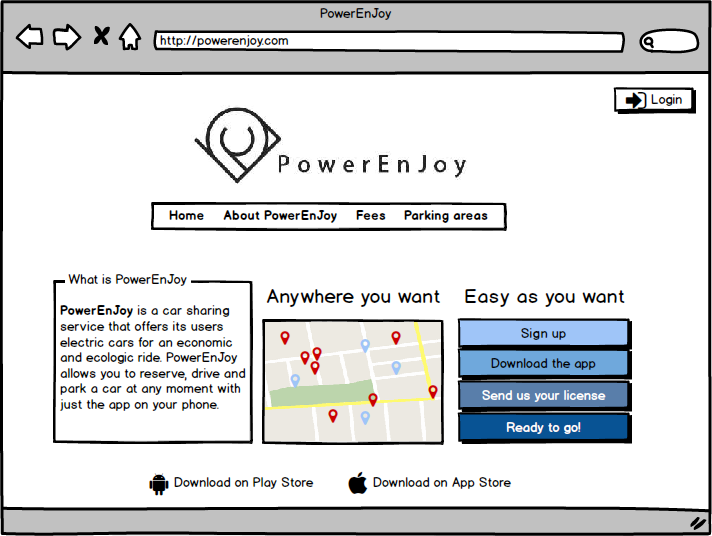
\includegraphics[scale=0.50]{img/mockups/Website.png}
			\caption{Website homepage}
			\label{fig:subim1}
		\end{subfigure}
		\begin{subfigure}{1\textwidth}
			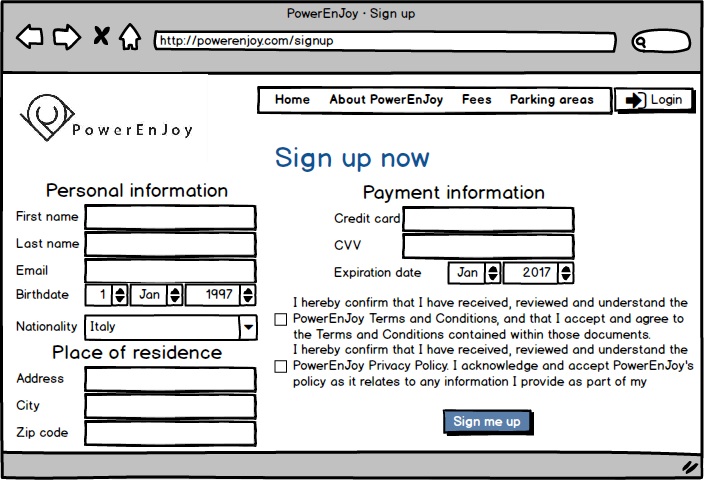
\includegraphics[scale=0.50]{img/mockups/Sign_up.png}
			\caption{Sign up on website}
			\label{fig:subim2}
		\end{subfigure}
		
		\caption{Website}
		\label{fig:image3}
	\end{figure}

	\paragraph{} Figure 3.a and 3.b shows, respectively, the website homepage from the standpoint of a guest and the sign up page. We haven't drawn the website mockup from the standpoint of a registered user since there are no more functionalities than those already present in the mobile app, as said above.



\FloatBarrier %to forbit images to enter the scenario chapter.